%----------------------------------------------------------------------------------------
%    PACKAGES AND THEMES
%----------------------------------------------------------------------------------------

\documentclass[aspectratio=169,xcolor=dvipsnames]{beamer}
\usetheme{SimplePlus}

\usepackage{hyperref}
\usepackage{graphicx}
\usepackage{booktabs}
\usepackage{amsmath}
\usepackage{tikz}
\usepackage{multirow}
\usepackage{rotating}
\usepackage{emoji}

\graphicspath{{../figures/}}

%----------------------------------------------------------------------------------------
%    TITLE PAGE
%----------------------------------------------------------------------------------------

\title{Evaluating Temporal Link Prediction methods to generate synthetic social networks data}
\subtitle{} %Using EvolveGCN on the Gab Dataset}

\author{Mattia Curri - Big Data Project}

\institute
{
    %Department of Computer Science\\
    %University
}
\date{\today}

%----------------------------------------------------------------------------------------
%    PRESENTATION SLIDES
%----------------------------------------------------------------------------------------

\begin{document}

\begin{frame}
	\titlepage
\end{frame}

% \begin{frame}{Overview}
% 	\tableofcontents
% \end{frame}

%------------------------------------------------
\section{Business Understanding}
%------------------------------------------------

\begin{frame}{Problem Statement}
	\begin{columns}[c]
		\column{0.55\textwidth}
		\begin{itemize}
			\item Social networks: critical for understanding modern online communities
			\item Risky users exploit platforms for malicious activities
			\item \textbf{Goal}: Temporal link prediction for social network analysis
		\end{itemize}

		\column{0.45\textwidth}
		\begin{block}{Objectives}
			\begin{enumerate}
				\item Predict future user connections
				\item Evaluate incremental learning
				\item Generate synthetic networks
			\end{enumerate}
		\end{block}
	\end{columns}
\end{frame}

\begin{frame}{Dataset: Gab Social Network}
	\begin{columns}[c]
		\column{0.5\textwidth}
		\begin{itemize}
			\item Platform: Gab (2016--2025)
			\item 6 temporal snapshots
			\item Posts + social network graphs
			\item BERT embeddings provided
		\end{itemize}

		\column{0.5\textwidth}
		\begin{table}
			\footnotesize
			\begin{tabular}{lr}
				\toprule
				\textbf{Property} & \textbf{Value} \\
				\midrule
				Total Posts       & 182,545        \\
				Unique Users      & 27,002         \\
				Snapshots         & 6              \\
				Time Span         & 2016--2025     \\
				\bottomrule
			\end{tabular}
		\end{table}
	\end{columns}
\end{frame}

\begin{frame}{Synthetic Dataset}
	\begin{columns}[c]
		\column{0.5\textwidth}
		\begin{block}{Synthetic Users}
			\begin{itemize}
				\item 3 batches: 400 + 400 + 200
				\item Total: 1,000 synthetic users
				\item 9,990 synthetic posts
				\item Pre-computed BERT embeddings
			\end{itemize}
		\end{block}

		\column{0.5\textwidth}
		\begin{alertblock}{Purpose}
			\begin{itemize}
				\item Test model generalization
				\item Generate synthetic network links
				\item Evaluate structural realism
			\end{itemize}
		\end{alertblock}
	\end{columns}

	\vspace{0.5em}
	\centering
	\footnotesize
	\textit{Pipeline: Real graph + synthetic embeddings $\rightarrow$ trained model $\rightarrow$ predicted edges}
\end{frame}

%------------------------------------------------
\section{Data Understanding}
%------------------------------------------------

\begin{frame}{Data Quality: Missing Values}
	\begin{columns}[c]
		\column{0.55\textwidth}
		\begin{table}
			\centering
			\begin{tabular}{lr}
				\toprule
				\textbf{Attribute} & \textbf{Missing \%} \\
				\midrule
				Language           & 0.48\%              \\
				All others         & 0.00\%              \\
				\bottomrule
			\end{tabular}
		\end{table}

		\begin{itemize}
			\item 99.52\% overall completeness
			\item No empty content posts
			\item 100\% snapshot consistency
		\end{itemize}

		\column{0.45\textwidth}
		\begin{table}
			\centering
			\footnotesize
			\begin{tabular}{lrrr}
				\toprule
				\textbf{Snapshot} & \textbf{Snap.} & \textbf{Incr.} & \textbf{Cov.} \\
				\midrule
				2016-2021         & 18,926         & 18,926         & 100\%         \\
				2022              & 13,108         & 32,034         & 100\%         \\
				2023              & 13,376         & 45,410         & 100\%         \\
				2024              & 13,400         & 58,810         & 100\%         \\
				Jan-Jul 25        & 44,878         & 103,688        & 100\%         \\
				Jul 25            & 78,857         & 182,545        & 100\%         \\
				\bottomrule
			\end{tabular}
		\end{table}
	\end{columns}
\end{frame}

\begin{frame}{Duplicate Content Analysis}
	\begin{columns}[c]
		\column{0.5\textwidth}
		\begin{table}
			\centering
			\begin{tabular}{lr}
				\toprule
				\textbf{Snapshot} & \textbf{Dup. \%} \\
				\midrule
				2016-2021         & 1.79\%           \\
				2022              & 3.02\%           \\
				2023              & 4.21\%           \\
				2024              & 4.20\%           \\
				Jan-Jul 25        & 7.52\%           \\
				Jul 25            & 10.04\%          \\
				\bottomrule
			\end{tabular}
		\end{table}

		\column{0.5\textwidth}
		\begin{itemize}
			\item Increasing duplicate rate over time
			\item No duplicate post IDs
			\item Each post has unique metadata
		\end{itemize}
	\end{columns}
\end{frame}

\begin{frame}{BERT Embeddings: Real vs Synthetic}
	\centering
	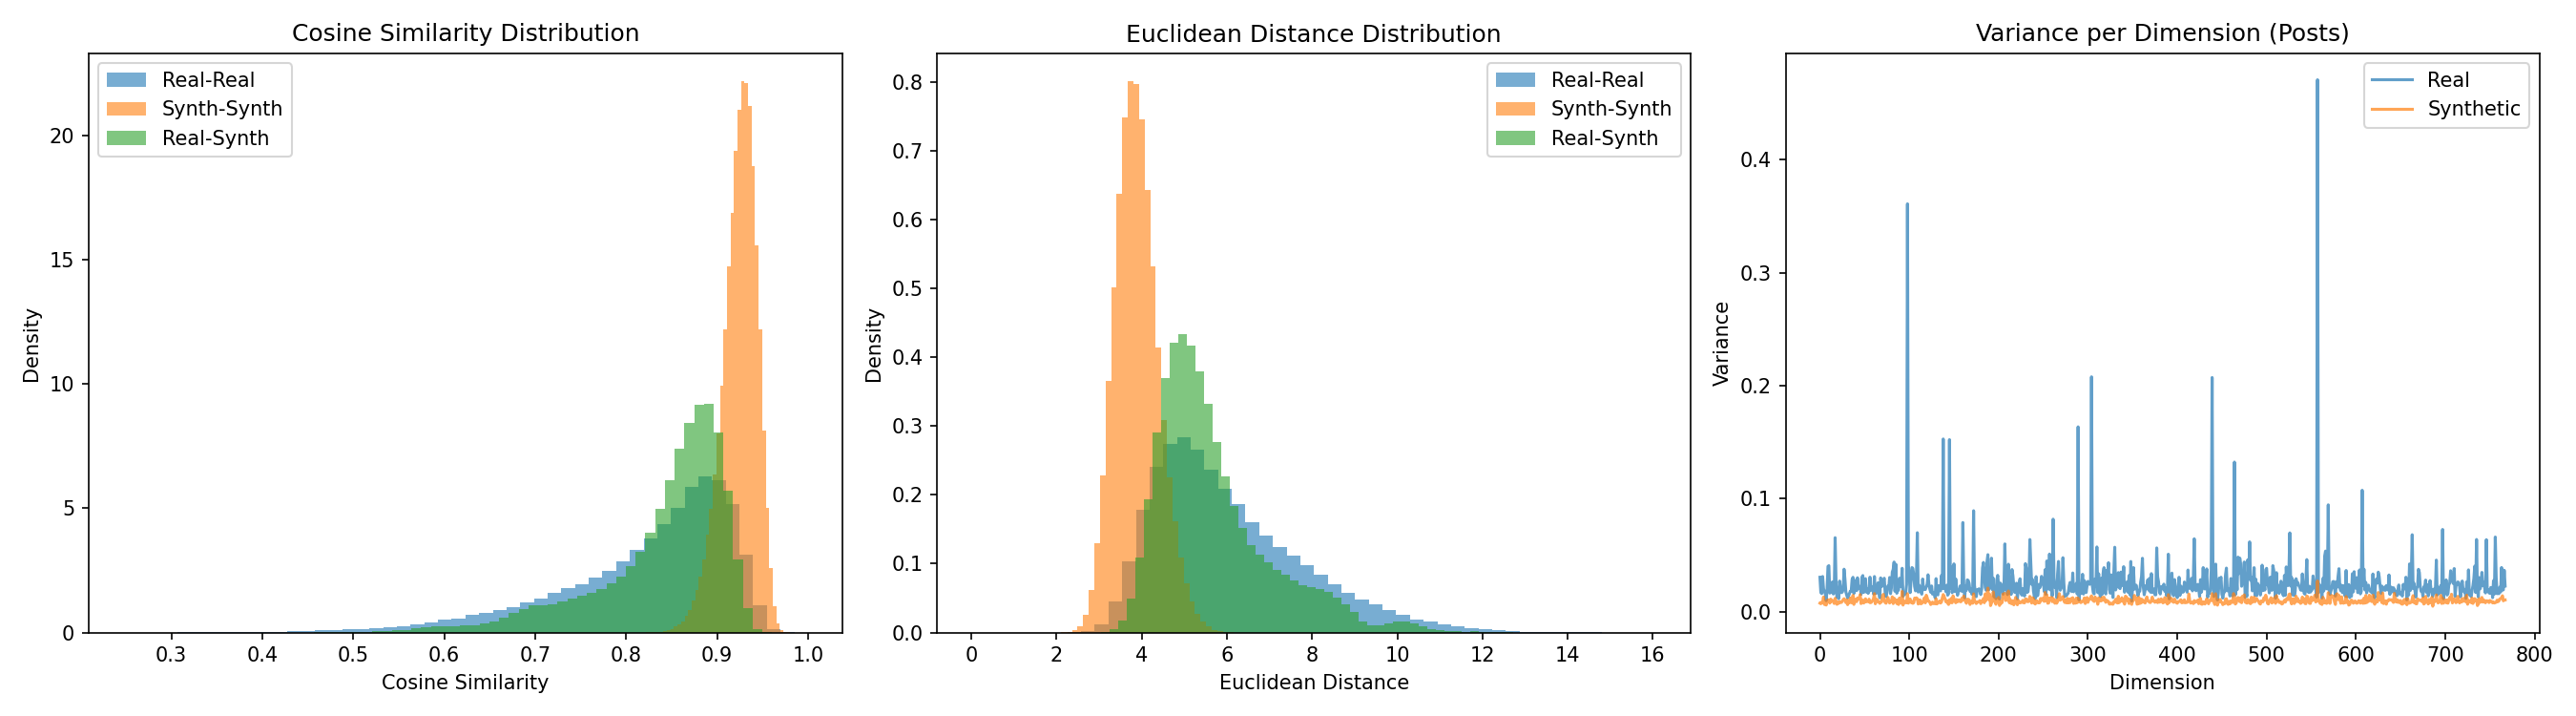
\includegraphics[width=0.9\textwidth]{embedding_comparison.png}
\end{frame}

\begin{frame}{Embedding Space Visualization}
	\centering
	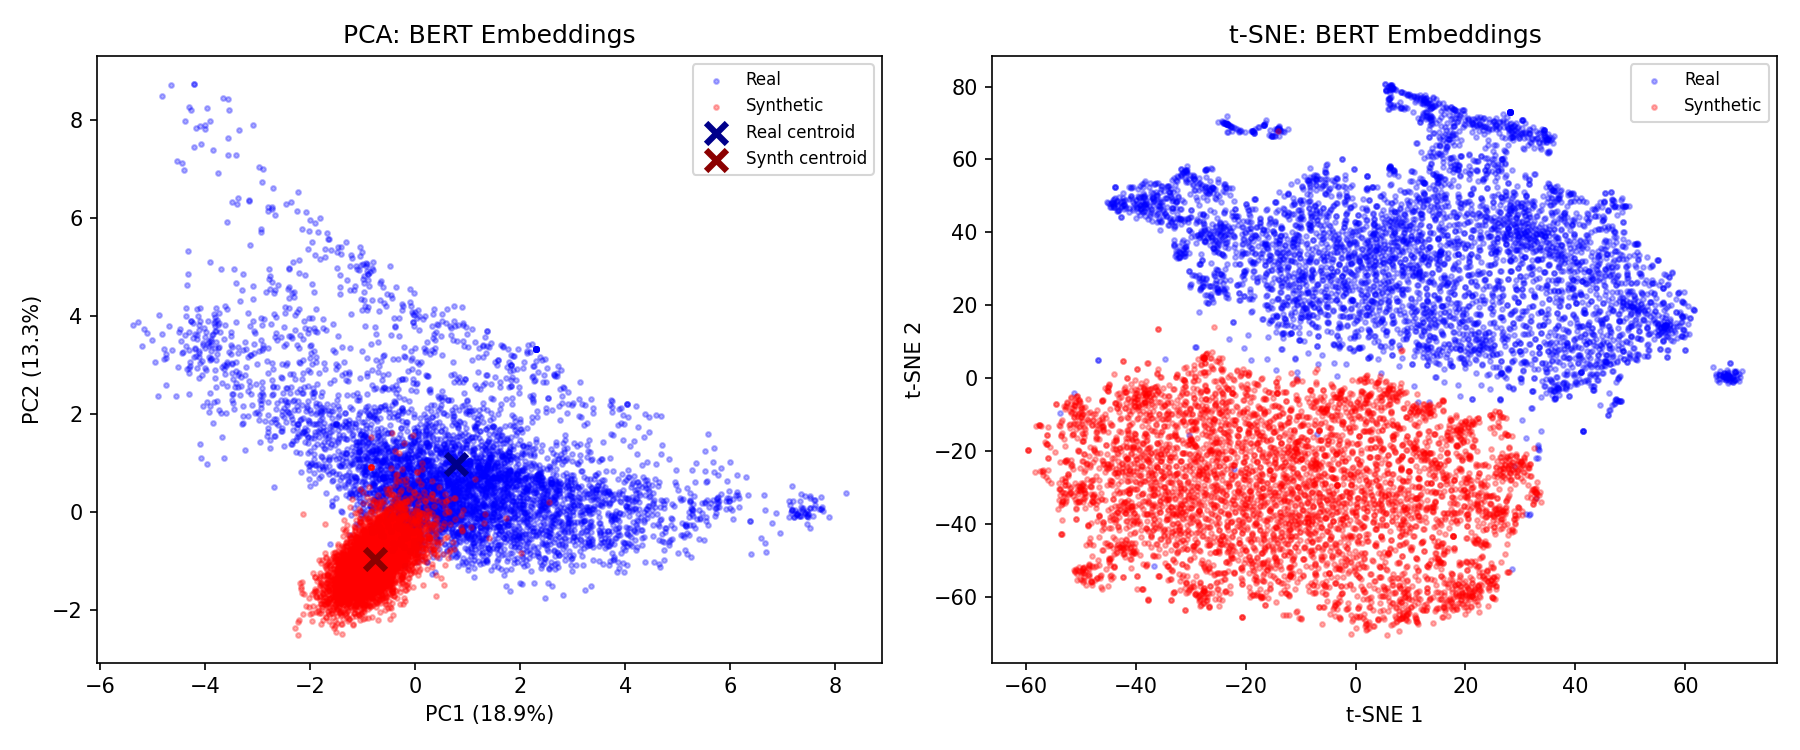
\includegraphics[width=0.95\textwidth]{embeddings_visualization_bert.png}
\end{frame}

\begin{frame}{User-Level Embedding Analysis}
	\centering
	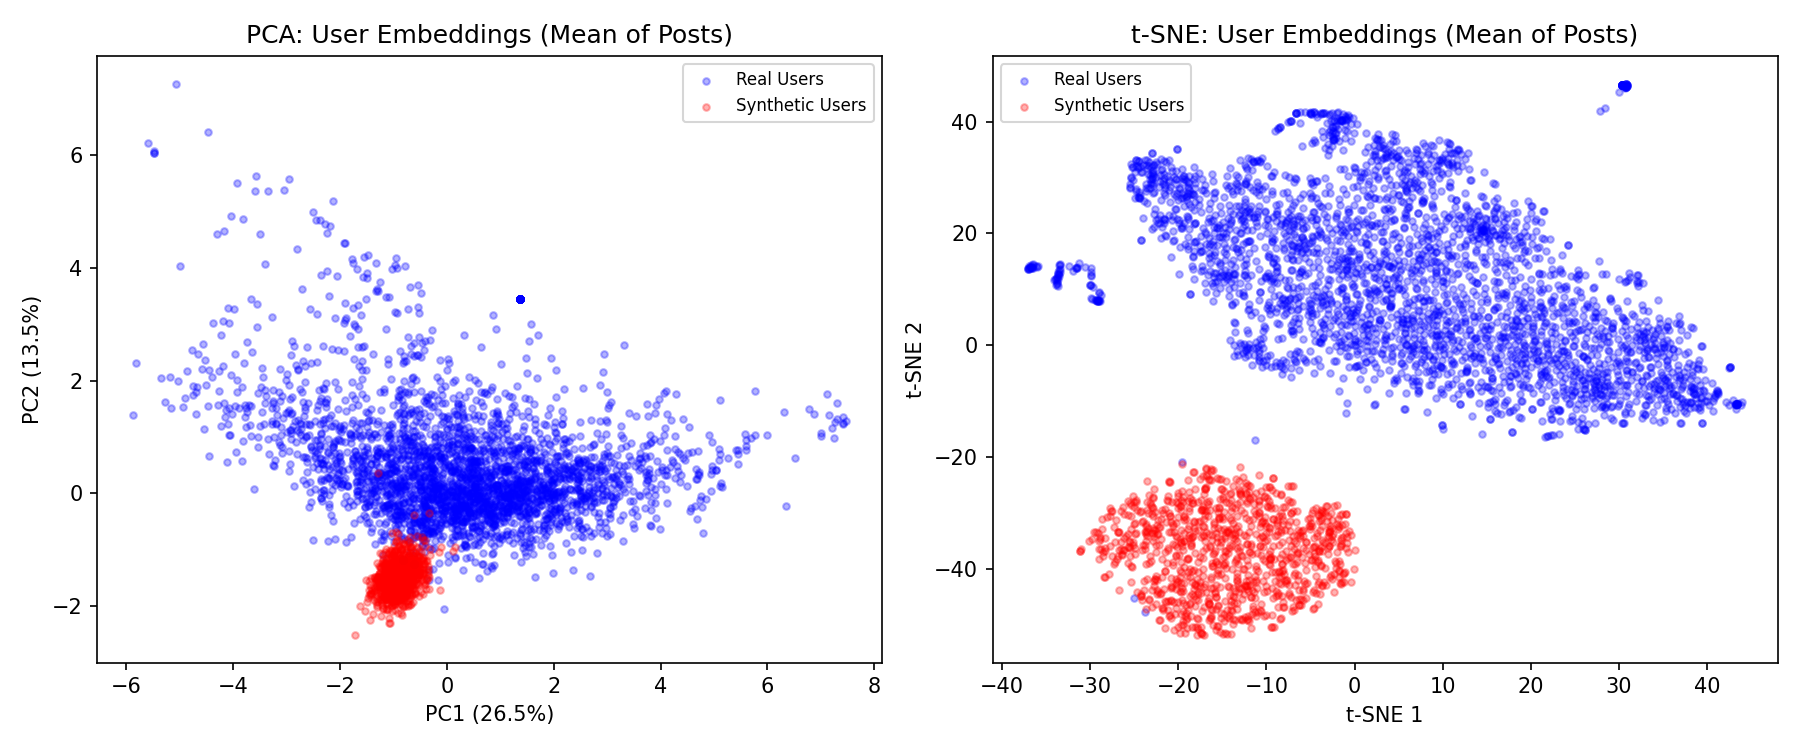
\includegraphics[width=0.95\textwidth]{user_embeddings_visualization.png}
\end{frame}

\begin{frame}{Embedding Statistics}
	\begin{columns}[c]
		\column{0.5\textwidth}
		\begin{table}
			\footnotesize
			\centering
			\begin{tabular}{lrr}
				\toprule
				\textbf{Metric}  & \textbf{Real} & \textbf{Synthetic} \\
				\midrule
				Posts            & 182,545       & 9,990              \\
				Cos. Sim. (mean) & 0.821         & 0.924              \\
				Cos. Sim. (std)  & 0.097         & 0.019              \\
				Variance         & 0.026         & 0.010              \\
				\bottomrule
			\end{tabular}
		\end{table}

		\column{0.5\textwidth}
		\begin{alertblock}{Key Finding}
			Synthetic users: variance ratio 11.23$\times$ lower than real users
		\end{alertblock}
	\end{columns}
\end{frame}

%------------------------------------------------
\section{Data Preparation}
%------------------------------------------------

\begin{frame}{Feature Construction}
	\begin{columns}[c]
		\column{0.5\textwidth}
		Node features from BERT embeddings:
		\[
			\mathbf{h}_u^{(t)} = \frac{1}{|P_u^{(t)}|} \sum_{p \in P_u^{(t)}} \text{BERT}(\text{content}_p)
		\]

		\begin{itemize}
			\item 768-dimensional feature vectors
			\item Temporal feature construction
			\item No data leakage
		\end{itemize}

		\column{0.5\textwidth}
		\begin{block}{Graph Structure}
			\begin{itemize}
				\item Directed graph $G_t = (V_t, E_t)$
				\item Cumulative edge assumption
				\item Sparse adjacency representation
			\end{itemize}
		\end{block}
	\end{columns}
\end{frame}

\begin{frame}{Adjacency Matrix Normalization}
	\[
		\hat{A}_t = \tilde{D}_t^{-\frac{1}{2}} \tilde{A}_t \tilde{D}_t^{-\frac{1}{2}}, \quad \tilde{A}_t = A_t + I
	\]

	\vspace{1em}

	\begin{columns}[c]
		\column{0.5\textwidth}
		\centering
		\textbf{Training Input:}
		\begin{itemize}
			\item Historical adjacency list $[\hat{A}_{t-k}, \ldots, \hat{A}_{t-1}]$
			\item Historical node features $[H_{t-k}, \ldots, H_{t-1}]$
			\item Node masks for active nodes
		\end{itemize}

		\column{0.5\textwidth}
		\centering
		\textbf{Training Output:}
		\begin{itemize}
			\item Edge pairs $(u, v)$
			\item Binary labels $y \in \{0, 1\}$
			\item Negative sampling
		\end{itemize}
	\end{columns}
\end{frame}

%------------------------------------------------
\section{Modeling}
%------------------------------------------------

\begin{frame}{EvolveGCN Architecture}
	\begin{columns}[c]
		\column{0.55\textwidth}
		\begin{block}{Key Innovation}
			RNN evolves GCN parameters instead of node embeddings
		\end{block}

		\textbf{Graph Convolution:}
		\[
			H_t^{(l+1)} = \sigma(\hat{A}_t H_t^{(l)} W_t^{(l)})
		\]

		\textbf{Weight Evolution (EvolveGCN-H):}
		\[
			W_t^{(l)} = \text{GRU}(H_t^{(l)}, W_{t-1}^{(l)})
		\]

		\column{0.45\textwidth}
		\begin{itemize}
			\item Handles new nodes at test time
			\item No requirement for static node sets
			\item Captures temporal dynamics
		\end{itemize}
	\end{columns}
\end{frame}

\begin{frame}{GCN Architecture Details}
	\begin{columns}[c]
		\column{0.5\textwidth}
		\textbf{GRCU Layers:}
		\begin{itemize}
			\item Layer 1: 768 $\rightarrow$ 128
			\item Layer 2: 128 $\rightarrow$ 64
		\end{itemize}

		\vspace{0.5em}

		\textbf{MLP Classifier:}
		\begin{itemize}
			\item Input: 128 (64 $\times$ 2 concatenated)
			\item Output: 2 logits
		\end{itemize}

		\vspace{0.5em}

		\textbf{Loss:}
		\[
			\mathcal{L} = -\frac{1}{N} \sum_{i=1}^N w_i \log(\hat{y}_i)
		\]

		\column{0.5\textwidth}
		\begin{alertblock}{Top-K Selection}
			\[
				\text{scores} = \frac{H_t^{(l)} \cdot s}{\|s\|}
			\]
			Select most relevant embeddings for weight evolution
		\end{alertblock}
	\end{columns}
\end{frame}

\begin{frame}{Training Pipelines}
	\begin{columns}[t]
		\column{0.48\textwidth}
		\begin{block}{Original Implementation}
			\begin{itemize}
				\item Sequence-based training
				\item All snapshots in single batch
				\item 50 epochs total
				\item GRU manages temporal flow
			\end{itemize}
		\end{block}

		\column{0.48\textwidth}
		\begin{block}{Incremental Implementation}
			\begin{itemize}
				\item Phase-based training
				\item One snapshot per phase
				\item 50 epochs per phase
				\item Weight transfer between phases
			\end{itemize}
		\end{block}
	\end{columns}

	\vspace{1em}

	\centering
	\textbf{Configurations:} LR $\in \{0.001, 0.0005\}$, NM $\in \{1, 2\}$
\end{frame}

%------------------------------------------------
\section{Evaluation}
%------------------------------------------------

\begin{frame}{Classification Results}
	\begin{table}
		\centering
		\footnotesize
		\begin{tabular}{llcccccc}
			\toprule
			 & \textbf{LR} & \textbf{NM} & \textbf{MAP}  & \textbf{AUC} & \textbf{Prec.} & \textbf{Rec.} & \textbf{F1}   \\
			\midrule
			\multirow{4}{*}{\rotatebox{90}{\textbf{Incr.}}}
			 & 0.001       & 1           & 0.78          & 0.78         & 0.25           & 0.49          & 0.33          \\
			 & 0.001       & 2           & 0.64          & 0.74         & 0.75           & 0.68          & 0.69          \\
			 & 0.0005      & 1           & 0.78          & 0.80         & 0.68           & 0.52          & 0.38          \\
			 & 0.0005      & 2           & 0.62          & 0.72         & 0.73           & 0.68          & 0.69          \\
			\midrule
			\multirow{4}{*}{\rotatebox{90}{\textbf{Orig.}}}
			 & 0.001       & 1           & \textbf{0.87} & 0.63         & \textbf{0.86}  & \textbf{0.86} & \textbf{0.86} \\
			 & 0.001       & 2           & 0.77          & 0.65         & 0.82           & 0.83          & 0.83          \\
			 & 0.0005      & 1           & 0.86          & 0.64         & 0.82           & 0.79          & 0.78          \\
			 & 0.0005      & 2           & 0.76          & 0.65         & 0.81           & 0.84          & 0.81          \\
			\bottomrule
		\end{tabular}
	\end{table}

	\vspace{0.5em}
	\centering
	\footnotesize
	\textit{Incr. = Incremental, Orig. = Original, LR = Learning Rate, NM = Negative Multiplier}
\end{frame}

\begin{frame}{Per-Class Metrics}
	\begin{table}
		\centering
		\footnotesize
		\begin{tabular}{llcccccccc}
			\toprule
			 & \textbf{LR} & \textbf{NM} & \multicolumn{3}{c}{\textbf{Class 0 (Non-link)}} & \multicolumn{3}{c}{\textbf{Class 1 (Link)}}                             \\
			\cmidrule(lr){4-6} \cmidrule(lr){7-9}
			 &             &             & P                                               & R                                           & F1   & P    & R    & F1   \\
			\midrule
			\multirow{4}{*}{\rotatebox{90}{\textbf{Incr.}}}
			 & 0.001       & 1           & 0.00                                            & 0.00                                        & 0.00 & 0.49 & 0.97 & 0.65 \\
			 & 0.001       & 2           & 0.77                                            & 0.92                                        & 0.83 & 0.73 & 0.44 & 0.55 \\
			 & 0.0005      & 1           & 0.85                                            & 0.04                                        & 0.08 & 0.51 & 0.99 & 0.67 \\
			 & 0.0005      & 2           & 0.77                                            & 0.90                                        & 0.83 & 0.69 & 0.47 & 0.56 \\
			\midrule
			\multirow{4}{*}{\rotatebox{90}{\textbf{Orig.}}}
			 & 0.001       & 1           & 0.89                                            & 0.83                                        & 0.86 & 0.84 & 0.89 & 0.87 \\
			 & 0.001       & 2           & 0.89                                            & 0.88                                        & 0.88 & 0.76 & 0.78 & 0.77 \\
			 & 0.0005      & 1           & 0.93                                            & 0.62                                        & 0.74 & 0.71 & 0.96 & 0.82 \\
			 & 0.0005      & 2           & 0.95                                            & 0.76                                        & 0.84 & 0.66 & 0.93 & 0.77 \\
			\bottomrule
		\end{tabular}
	\end{table}

	\vspace{0.3em}
	\footnotesize
	\begin{itemize}
		\item Original: balanced class prediction across all configs
		\item Incremental (NM=1): severe class imbalance, predicts mostly Class 1
	\end{itemize}
\end{frame}

\begin{frame}{GCN Embeddings: Original Implementation}
	\centering
	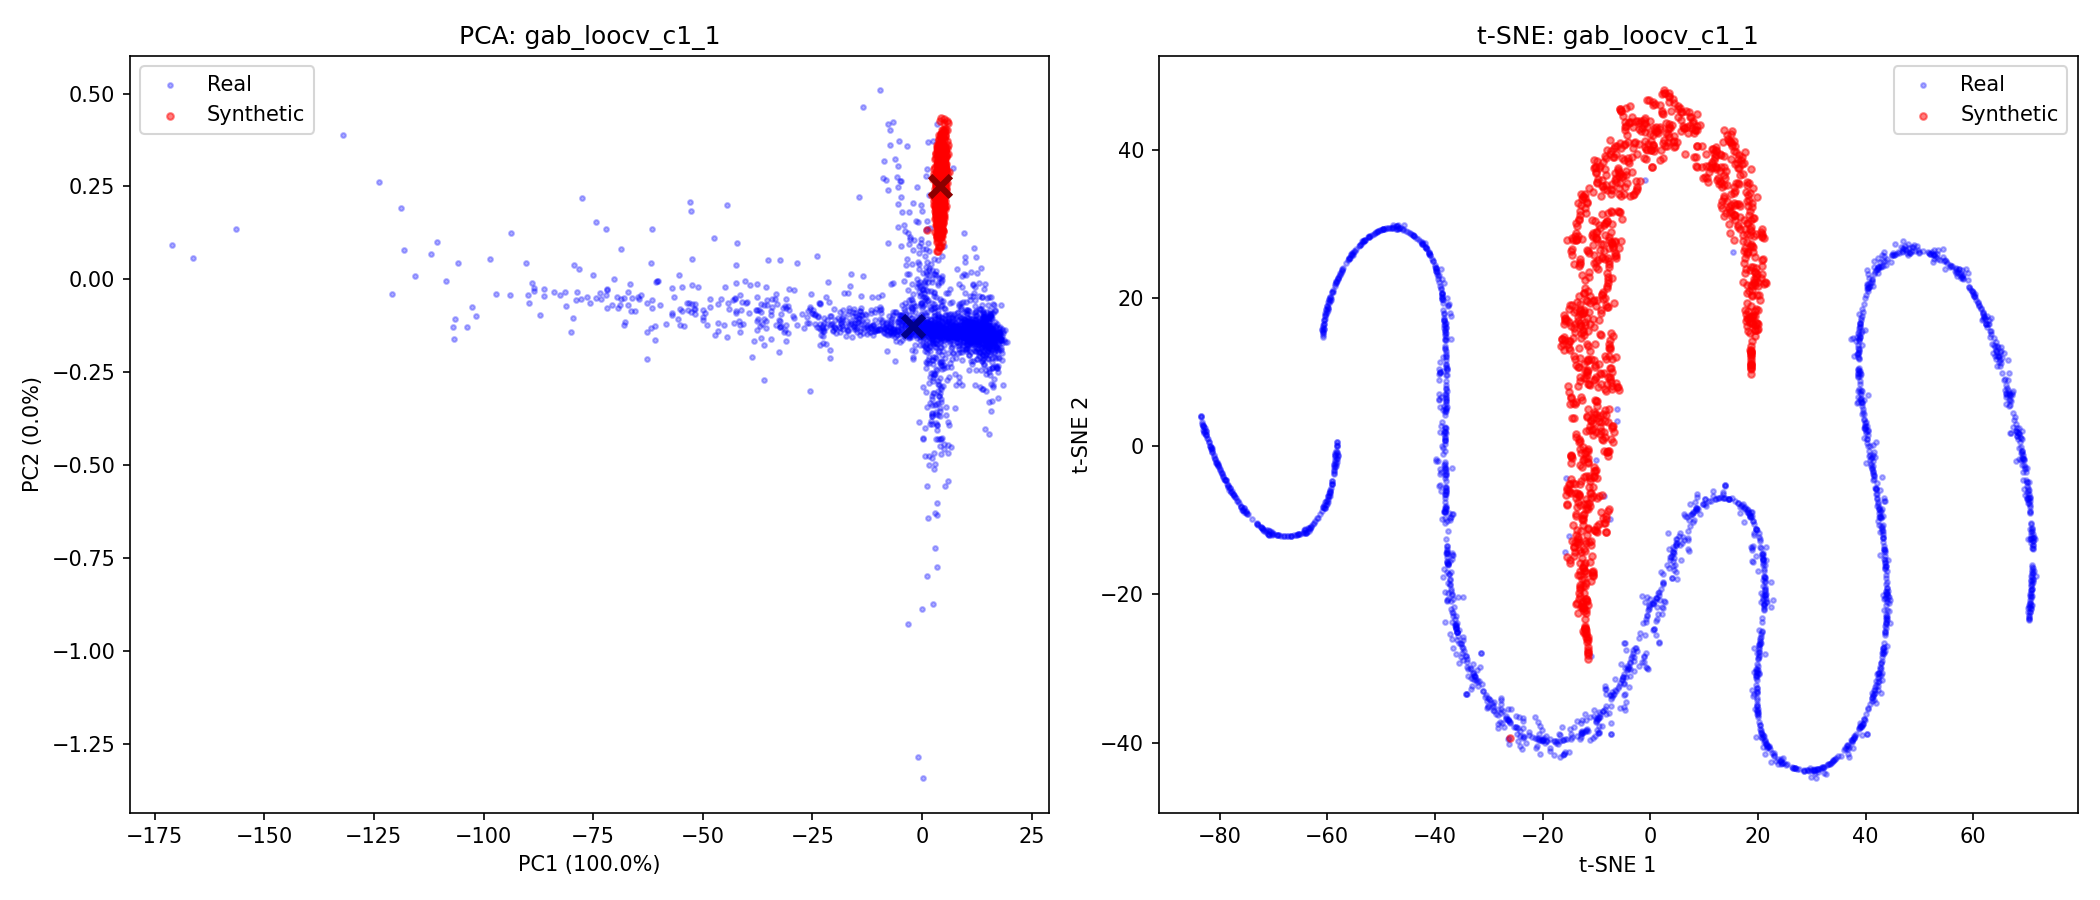
\includegraphics[width=0.95\textwidth]{gab_loocv_c1_1_gcn_visualization.png}
\end{frame}

\begin{frame}{GCN Embeddings: Incremental Implementation}
	\centering
	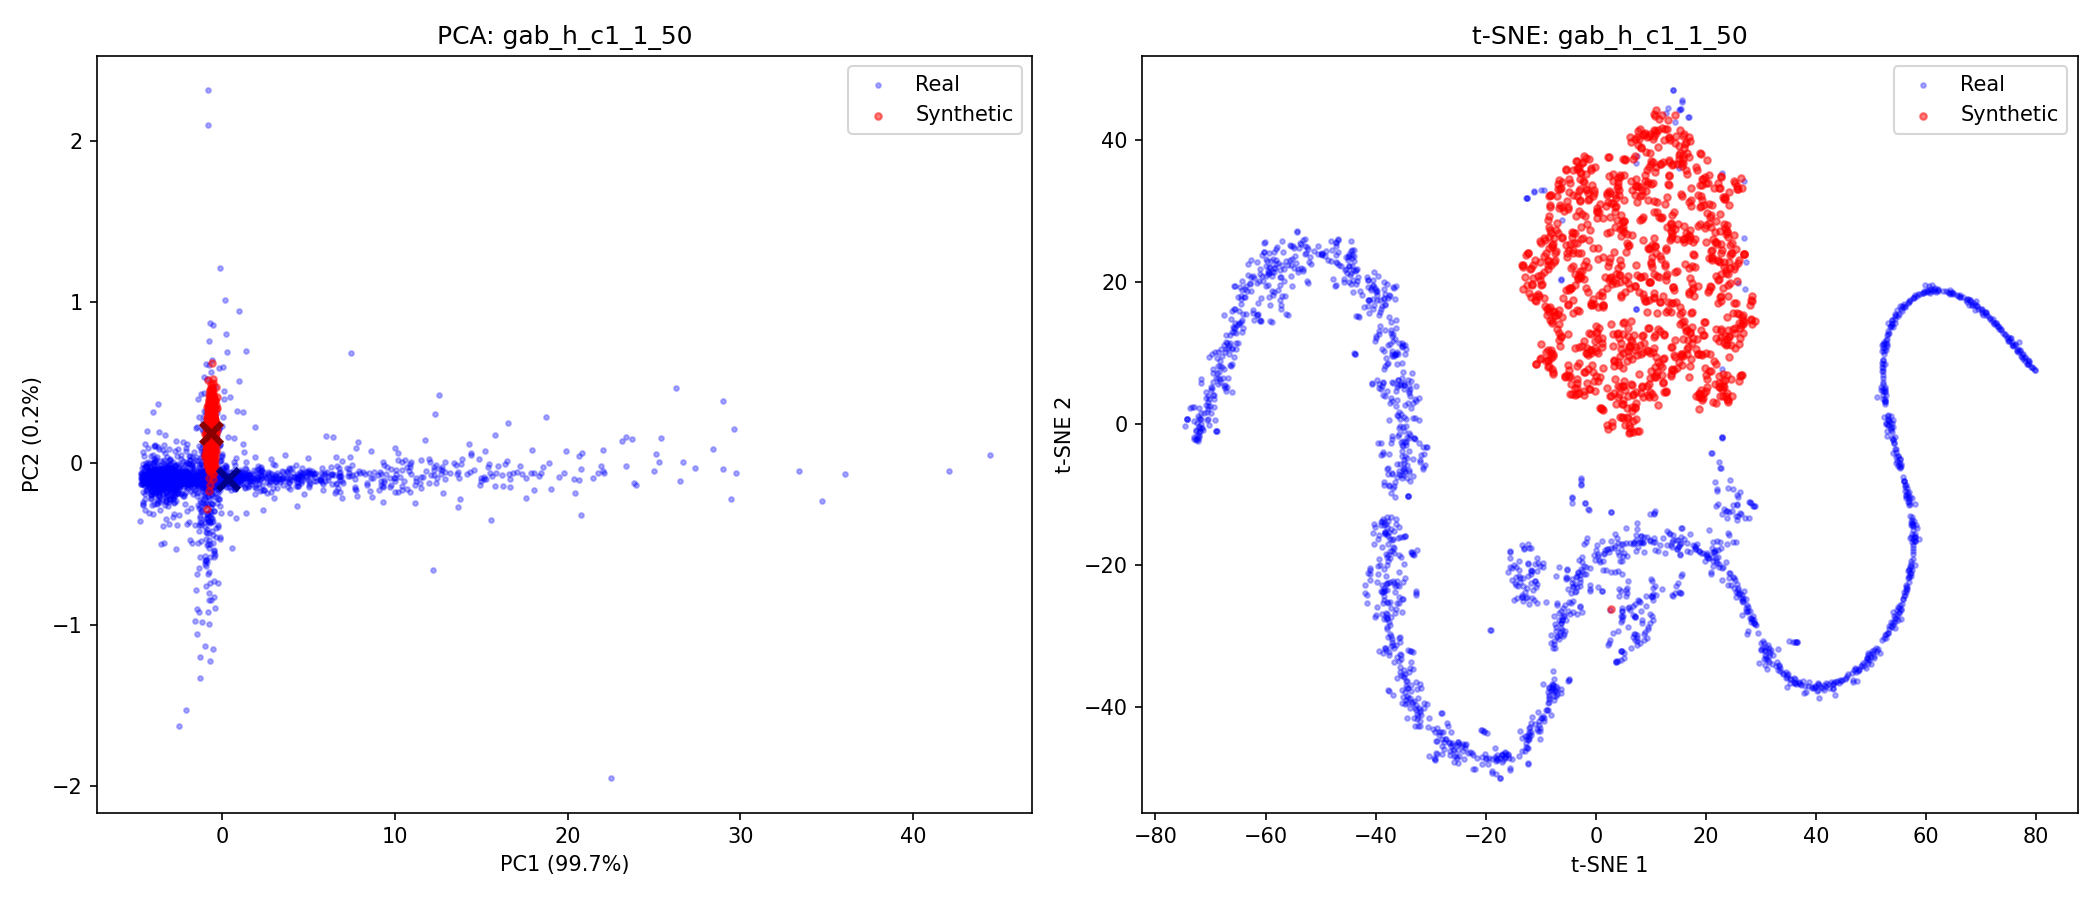
\includegraphics[width=0.95\textwidth]{gab_h_c1_1_50_gcn_visualization.png}
\end{frame}

\begin{frame}{All Configurations: Original}
	\centering
	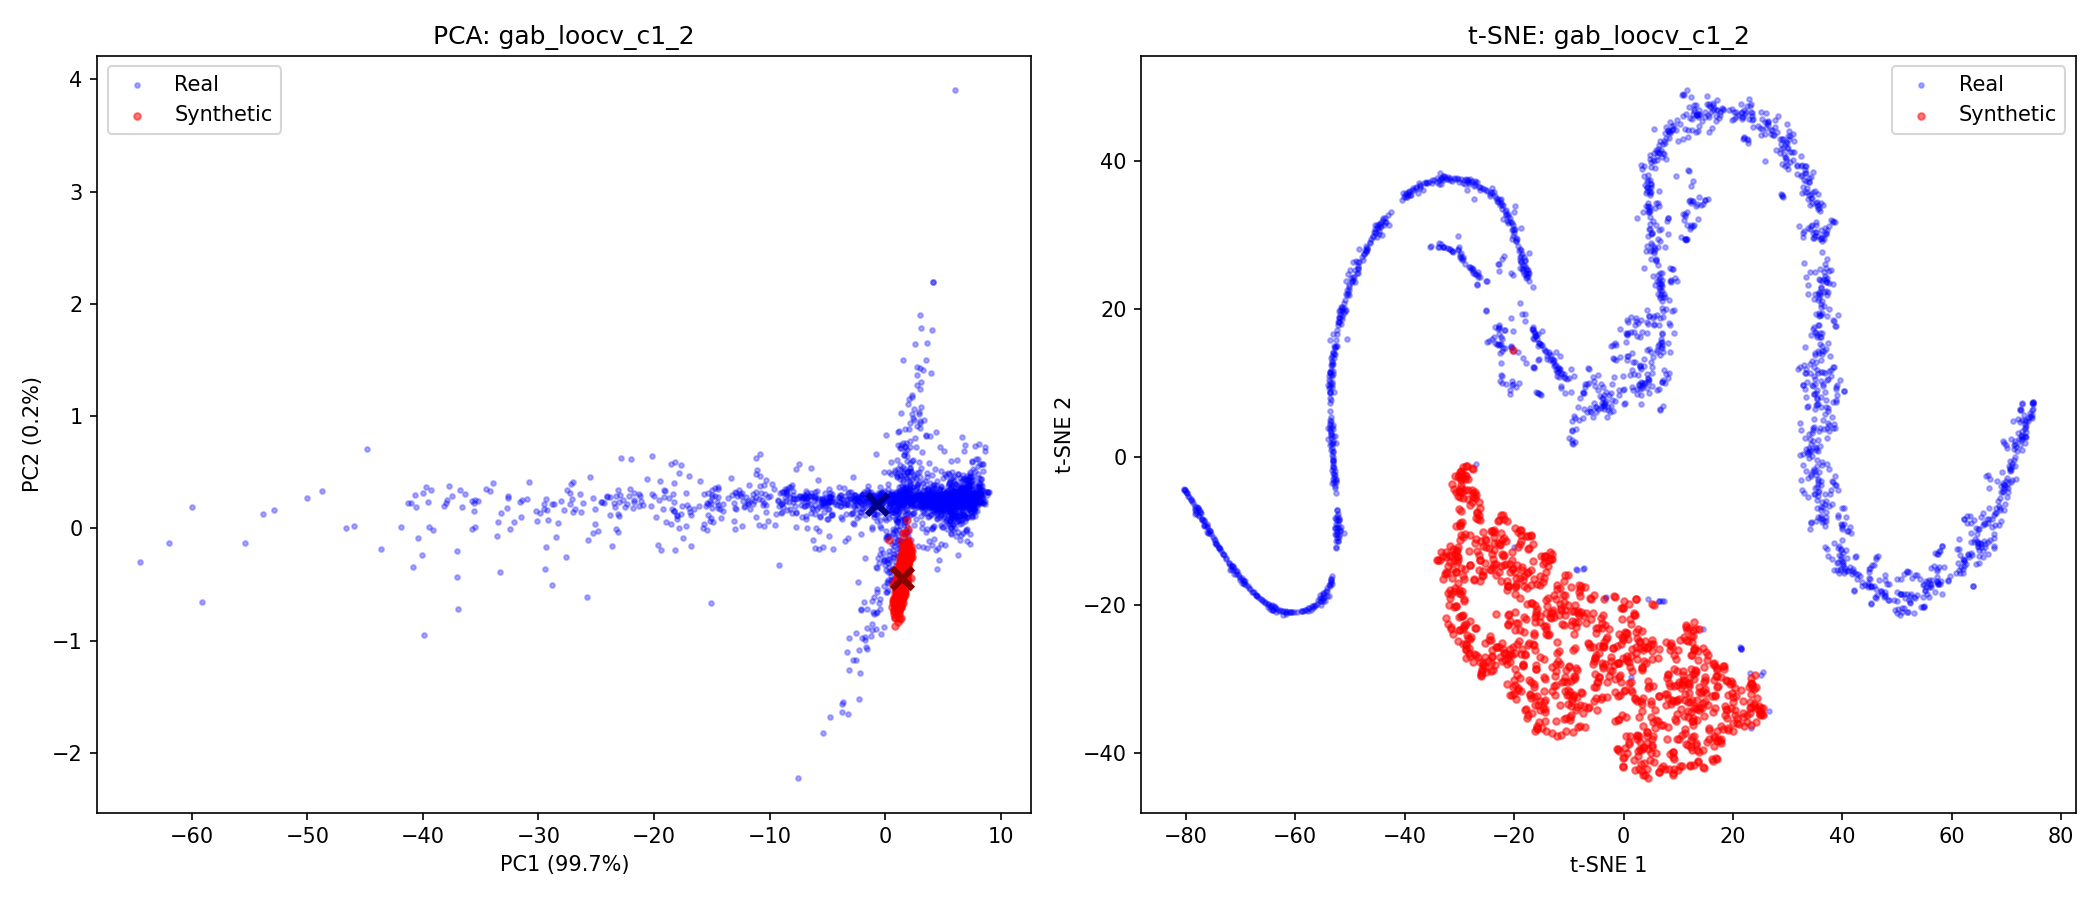
\includegraphics[width=0.85\textwidth]{gab_loocv_c1_2_gcn_visualization.png}
\end{frame}

\begin{frame}{All Configurations: Incremental}
	\centering
	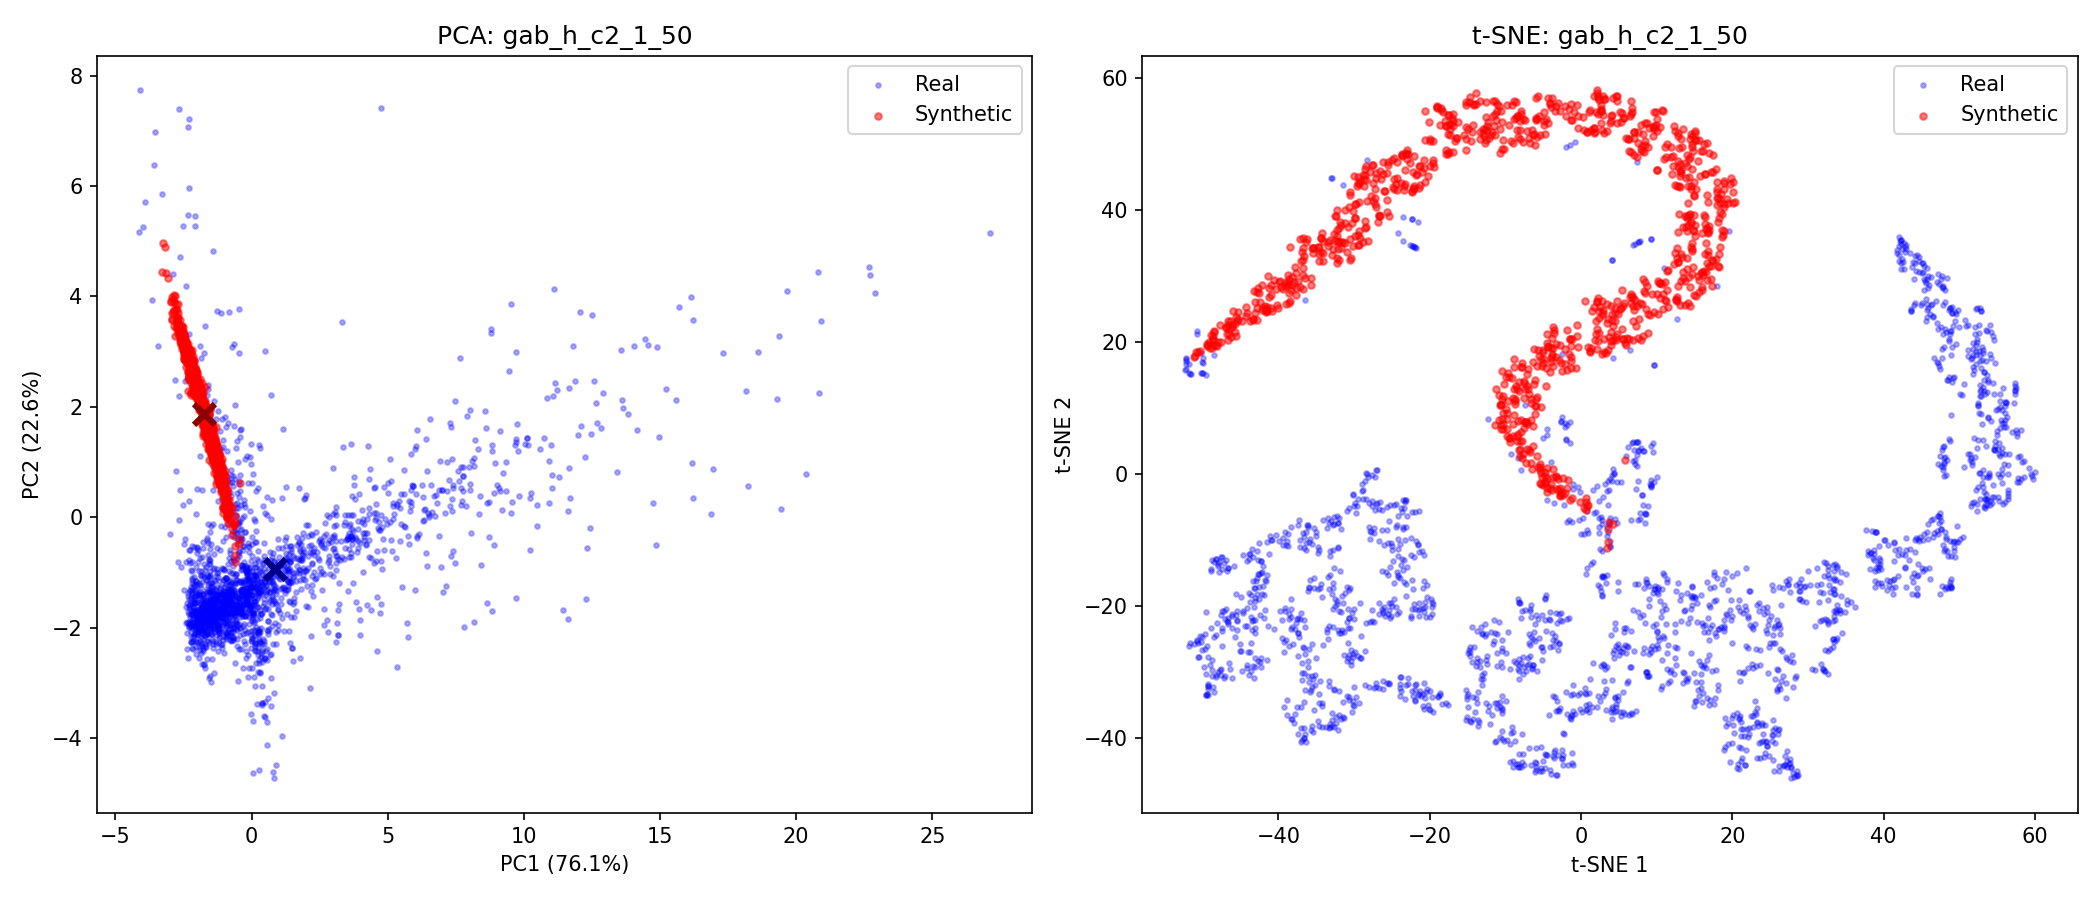
\includegraphics[width=0.85\textwidth]{gab_h_c2_1_50_gcn_visualization.png}
\end{frame}

\begin{frame}{PCA Statistics}
	\begin{table}
		\centering
		\scriptsize
		\begin{tabular}{llcccc}
			\toprule
			 & \textbf{Config} & \textbf{PC1} & \textbf{PC2} & \textbf{Total} & \textbf{Centroid} \\
			\midrule
			\multirow{4}{*}{\rotatebox{90}{\textbf{Orig.}}}
			 & LR=0.001, NM=1  & 99.98\%      & 0.01\%       & 100.00\%       & 6.29              \\
			 & LR=0.001, NM=2  & 99.71\%      & 0.23\%       & 99.94\%        & 2.33              \\
			 & LR=0.0005, NM=1 & 95.99\%      & 3.39\%       & 99.38\%        & 2.06              \\
			 & LR=0.0005, NM=2 & 99.96\%      & 0.03\%       & 100.00\%       & 6.65              \\
			\midrule
			\multirow{4}{*}{\rotatebox{90}{\textbf{Incr.}}}
			 & LR=0.001, NM=1  & 99.65\%      & 0.21\%       & 99.86\%        & 1.01              \\
			 & LR=0.001, NM=2  & 99.39\%      & 0.57\%       & 99.96\%        & 3.41              \\
			 & LR=0.0005, NM=1 & 76.13\%      & 22.61\%      & 98.74\%        & 3.84              \\
			 & LR=0.0005, NM=2 & 91.20\%      & 8.47\%       & 99.67\%        & 4.78              \\
			\bottomrule
		\end{tabular}
	\end{table}

	\vspace{0.3em}
	\begin{alertblock}{Key Finding}
		Original: Dimensional collapse (PC1 $\approx$ 96-100\%)\\
		Incremental (LR=0.0005, NM=1): Richer embedding space (PC1 = 76\%)
	\end{alertblock}
\end{frame}

\begin{frame}{Graph Metrics Comparison}
	\begin{table}
		\centering
		\begin{tabular}{lcccc}
			\toprule
			\textbf{Network}                & \textbf{Avg Deg} & \textbf{Mod.} & \textbf{Avg Path} & \textbf{Clust.} \\
			\midrule
			Facebook                        & 43.69            & 0.83          & 3.62              & 0.61            \\
			Twitter                         & 21.75            & 0.80          & 4.90              & 0.57            \\
			Google+                         & 127.06           & 0.47          & 3.32              & 0.49            \\
			\textbf{Gab (Ours)}             & 32.11            & 0.27          & 3.04              & 0.08            \\
			\midrule
			Synthetic (Incr. LR=.0005 NM=1) & 220.35           & -0.001        & 1.02              & 0.59            \\
			\bottomrule
		\end{tabular}
	\end{table}

	\vspace{0.5em}
	\begin{itemize}
		\item Synthetic: over-dense, no community structure (modularity $\approx$ 0)
		\item Gab: lower clustering than mainstream networks
	\end{itemize}
\end{frame}

\begin{frame}{Key Observations}
	\begin{columns}[c]
		\column{0.5\textwidth}
		\begin{block}{Original Implementation}
			\begin{itemize}
				\item Best MAP: 0.87
				\item Best F1: 0.86
				\item Severe oversmoothing
				\item No synthetic connections
			\end{itemize}
		\end{block}

		\column{0.5\textwidth}
		\begin{block}{Incremental Implementation}
			\begin{itemize}
				\item Best AUC: 0.80
				\item Richer embeddings
				\item Attempts synthetic links
				\item Poor structural fidelity
			\end{itemize}
		\end{block}
	\end{columns}
\end{frame}

%------------------------------------------------
\section{Conclusion}
%------------------------------------------------

\begin{frame}{Achievement of Goals}
	\begin{columns}[c]
		\column{0.5\textwidth}
		\begin{exampleblock}{Achieved}
			\begin{itemize}
				\item Temporal link prediction model
				\item Quantitative evaluation
				\item Embedding space analysis
			\end{itemize}
		\end{exampleblock}

		\column{0.5\textwidth}
		\begin{alertblock}{Failed}
			\begin{itemize}
				\item Realistic synthetic networks
				\item Generalization to synthetic users
			\end{itemize}
		\end{alertblock}
	\end{columns}
\end{frame}

\begin{frame}{Limitations}
	\begin{enumerate}
		\item \textbf{Embedding Mismatch}: Synthetic users too homogeneous (variance ratio 11.23$\times$)

		\item \textbf{Oversmoothing}: Dimensional collapse in GCN layers

		\item \textbf{Cumulative Edge Assumption}: Does not reflect unfollowing behavior
	\end{enumerate}

	\vspace{1em}

	\centering
	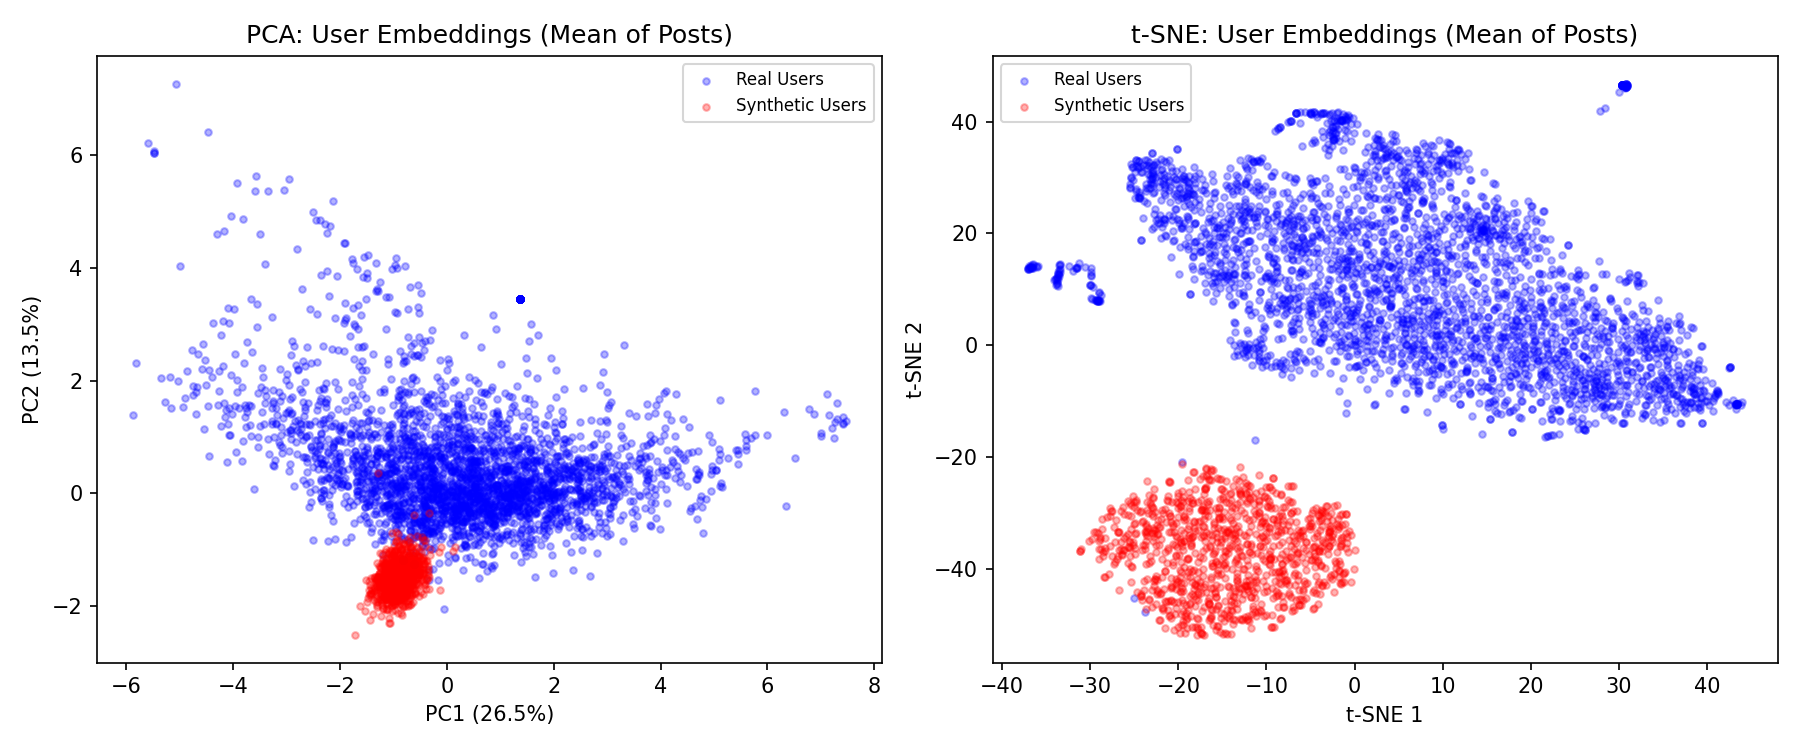
\includegraphics[width=0.6\textwidth]{user_embeddings_visualization.png}
\end{frame}

\begin{frame}{Future Work}
	\begin{enumerate}
		\item \textbf{Mitigate Oversmoothing}
		      \begin{itemize}
			      \item Jumping knowledge networks
			      \item APPNP-style propagation
			      \item Fewer GCN layers
		      \end{itemize}

		\item \textbf{Improve Synthetic Data}
		      \begin{itemize}
			      \item Diverse generation prompts
			      \item Embedding perturbation
		      \end{itemize}

		\item \textbf{Alternative Models}
		      \begin{itemize}
			      \item Other temporal GNN architectures
			      \item Attention-based approaches
		      \end{itemize}
	\end{enumerate}
\end{frame}

\begin{frame}
	\Huge{\centerline{\textbf{Thank You} \emoji{rocket}}}
	\vspace{1em}
	\large{\centerline{Questions?}}
\end{frame}

%----------------------------------------------------------------------------------------

\end{document}
